\documentclass{beamer}    
\usepackage{amsmath}
\usepackage{stmaryrd}
\usepackage{wasysym}
\usepackage[absolute,overlay]{textpos}
\usepackage{hyperref}
\usepackage{multicol}
\usepackage[font=small]{caption}
\setbeamercolor{framesource}{fg=gray}
\setbeamerfont{framesource}{size=\tiny}
\usepackage[utf8]{inputenc}
\usepackage{algpseudocode}
\usepackage{booktabs}
\usepackage{multirow}
\usetheme{Madrid}

\setlength{\abovecaptionskip}{0pt}
%\usepackage{caption}
%\captionsetup[figure]{labelformat=empty}

\newcommand{\fullhline}[0]{\noindent\makebox[\linewidth]{\rule{\paperwidth}{0.4pt}}}

\newcommand{\source}[1]{\begin{textblock*}{4cm}(8.7cm,8.3cm)
    \begin{beamercolorbox}[ht=0.5cm,right]{framesource}
        \usebeamerfont{framesource}\usebeamercolor[fg]{framesource} Source: {#1}
    \end{beamercolorbox}
\end{textblock*}}
\newcommand{\stateset}[0]{\mathcal{S}}
\newcommand{\actionset}[0]{\mathcal{A}}
\newcommand{\rewardset}[0]{\mathbb{R}}
\DeclareMathOperator*{\argmax}{argmax}

\newcommand\blfootnote[1]{%
  \begingroup
  \renewcommand\thefootnote{}\footnote{#1}%
  \addtocounter{footnote}{-1}%
  \endgroup
}

\AtBeginSection[]{
  \begin{frame}
  \vfill
  \centering
  \begin{beamercolorbox}[sep=8pt,center,shadow=true,rounded=true]{title}
    \usebeamerfont{title}\insertsectionhead\par%
  \end{beamercolorbox}
  \vfill
  \end{frame}
}

 
%Information to be included in the title page:
\title[] %optional
{Authorship Identification}
 
\author[]{Nick Fireman}
 
\date{April 15, 2021}

\begin{document}
\frame{\titlepage}

% \begin{frame}
% \frametitle{Table of Contents}
% \tableofcontents
% \end{frame}
\section{Background}

\begin{frame}{\secname: Authorship Identification}
\begin{itemize}
\item 
Authorship identification can be viewed as a type of \textbf{classification}.
    \begin{itemize}
    \item 
    Given a fixed set of potential authors and a passage, which author wrote the passage?
    \end{itemize}

~\\

\item
Previous approaches used language-specific statistical analysis inspired by NLP and \textbf{stylometry}:
\begin{itemize}
    \item Linguistic complexity
    \item Part of speech frequencies
    \item Function word frequencies (pronouns, prepositions, conjunctions) % words that don't affect the meaning of the passage, and so may reflect the personal flair of the author, which may identify them
\end{itemize}

\end{itemize}
\end{frame}

\begin{frame}{\secname: Word Embeddings}
\begin{itemize}
\item 
Let $W$ be a set of English words or \textbf{tokens}.

\begin{itemize}
    \item Tokens can include punctuation, numbers, and contractions (\texttt{n't}, \texttt{'re}).
\end{itemize}

~\\

\item 
A \textbf{word embedding} $e: W \rightarrow \mathbb{R}^n$ is a numeric representation of words that aims to \textbf{preserve meaning}.
    \begin{itemize}
        \item $W$ is the \textbf{vocabulary} of the embedding.
        \item $n$ is the \textbf{dimension} of the embedding.
    \end{itemize}

~\\

\item Similar words are mapped to similar vectors (in Euclidean distance).
    \begin{itemize}
    \item
    If $w, w' \in W$ and $| e(w') - e(w) |$ is small, then $w'$ is similar to $w$.
    \end{itemize}
\end{itemize}
\end{frame}

\begin{frame}{\secname: GloVe}
\begin{itemize}
    \item GloVe is an \textbf{unsupervised} algorithm which produces a word embedding from a text dataset.
    
    \item Motivated by \textbf{word co-occurrence}: two words consistently appearing near each other.
    
    \item GloVe embeddings preserve \textbf{analogical} relationships between words:
\end{itemize}

\begin{columns}
\begin{column}{0.5\textwidth}
\centering
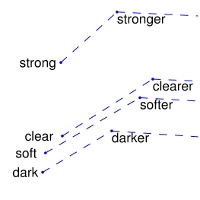
\includegraphics[scale=7]{images/glove-1.jpg}
\end{column}
\begin{column}{0.5\textwidth}
\centering
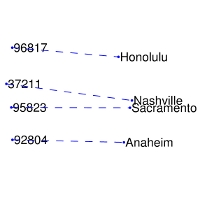
\includegraphics[scale=8]{images/glove-2.jpg}
\end{column}
\end{columns}
\blfootnote{\textbf{Figures}: https://nlp.stanford.edu/projects/glove/}
\end{frame}

\begin{frame}{\secname: RNN}
\begin{itemize}
\item 
Let $e: W \rightarrow \mathbb{R}^n$ be an $n$-dimensional word embedding.

\item
The embedding $e$ lets us map a passage to a sequence of vectors:
\begin{itemize}
\item 
Passages are \textbf{tokenized} into a sequence $\{w_1, w_2, ..., w_t\}$ in $W$.

\item
Then \textbf{embedded} to a sequence $\{e(w_1), e(w_2), ..., e(w_t)\}$ in $\mathbb{R}^n$.
\end{itemize}

\item
The RNN architecture is well-suited for understanding sequential data:
\end{itemize}

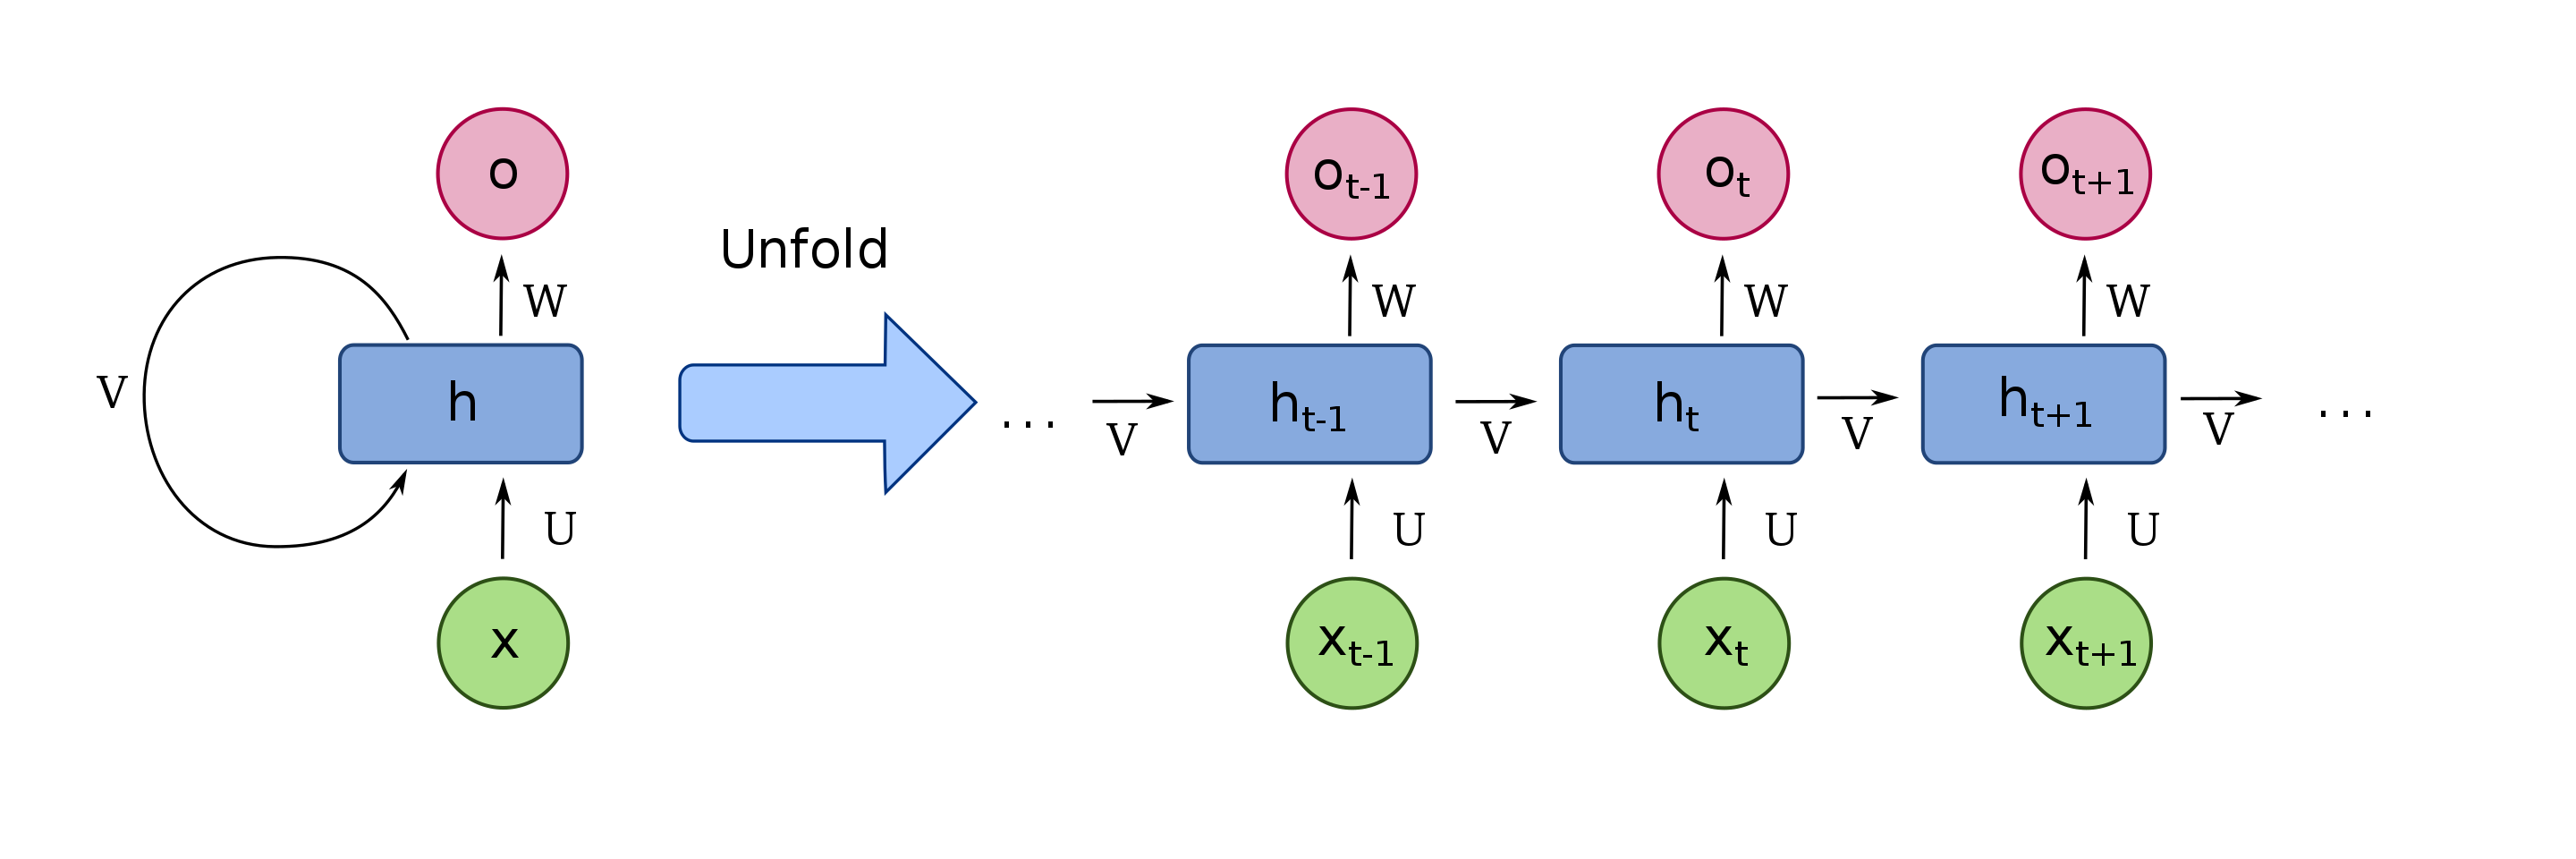
\includegraphics[width=\textwidth]{images/rnn.png}
\blfootnote{\textbf{Figure}: Wikipedia}
\end{frame}

\begin{frame}{\secname: Architecture}
\begin{itemize}

\item This project attempts to classify \textbf{short passages} written by the two authors Charles Dickens and Mark Twain.

\item 
Our high-level approach to author identification:

    \begin{itemize}
    \item 
    Extract passages from a literary dataset for training and testing.
    
    \item
    Use a word embedding to map each passage to a sequence of vectors.
    
    \item 
    Use an RNN to classify the sequential data.
    \end{itemize}
\end{itemize}
\end{frame}

\section{Datasets}

\begin{frame}{\secname: Project Gutenberg}
\begin{itemize}
\item 
Project Gutenberg hosts public domain English literature.

\item 
A 2015 research work\footnote{
Shibamouli Lahiri. “Complexity of Word Collocation Networks: A Preliminary Structural Analysis”}
collected and \textbf{cleaned} 3,036 books on PG
into a single dataset.
    \begin{itemize}
    \item Metadata, licenses, and transcribers' notes were removed from the original documents.
    
    \end{itemize}
    
\item
47 books by Mark Twain (3.3 million tokens). 

\item
61 books by Charles Dickens (7.1 million tokens).

\end{itemize}
\end{frame}

\begin{frame}{\secname: Pretrained GLoVE embeddings}
\begin{itemize}
\item 
The researchers who introduced GloVe also provide \textbf{pretrained} word embeddings produced by GloVe.

\item 
Embedding 1 (\texttt{6B.50d}) trained on 6 billion tokens from Wikipedia.
    \begin{itemize}
        \item Dimension 50.
        \item 400K-word vocabulary.
    \end{itemize}

\item
Embedding 2 (\texttt{42B.300d}) trained on 42 billion tokens from Common Crawl.
    \begin{itemize}
        \item Dimension 300.
        \item 1.9M-word vocabulary.
    \end{itemize}

\end{itemize}
\end{frame}

\section{Experiments}

\begin{frame}[fragile]{\secname: Challenges}
\begin{itemize} 

\item
Dickens (1812-1870) and Twain (1835-1910) were contemporaries, meaning they may have a similar writing style.

\item
19th-century writing may not be accurately captured by pretrained GloVe models trained on 21st-century language.

\item
12,361 tokens parsed did not lie in the GloVe vocabulary:

\begin{verbatim}
    cripplewayboo 
    davenportseseses
    methoozellers 
    schnorkel
    summonsizzing
    witchingest
\end{verbatim}

\end{itemize}
\end{frame}

\begin{frame}{\secname: Hyperparameter Tuning}
\begin{itemize}
\item A round of 18 experiments was held for \textbf{hyperparameter tuning}.
\begin{itemize}
\item 
2 pretrained GloVe embeddings: \texttt{6B.50d}, \texttt{42B.300d}.

\item
3 RNN hidden sizes: 25, 50, 100.

\item
3 learning rates: 0.0005, 0.001, 0.005.

\end{itemize}

\item
For each experiment:
\begin{itemize}
    \item 40,000 training passages and 10,000 testing passages are sampled from the works of each author.
    \item Each passage is 30 tokens.
    \item The model is trained for 100 epochs, with testing every 10 epochs.
\end{itemize}

\end{itemize}
\end{frame}

\begin{frame}{\secname: \texttt{6B.50d} GloVe}
% Please add the following required packages to your document preamble:
% \usepackage{booktabs}
% \usepackage{multirow}
\begin{table}[]
\begin{tabular}{@{}|c|c|c|c|c|@{}}
\toprule
\textbf{GLoVE}            & \textbf{Hidden Size} & \textbf{LR} & \textbf{Peak Test Acc.} & \textbf{Final Acc.} \\ \midrule
\multirow{9}{*}{6B.50d}   & \multirow{3}{*}{25}  & 0.0005      & 0.7597 (90 epochs)      & 0.7586              \\ \cmidrule(l){3-5} 
                          &                      & 0.001       & 0.7854 (100 epochs)     & 0.7854              \\ \cmidrule(l){3-5} 
                          &                      & 0.005       & 0.7972 (100 epochs)     & 0.7972              \\ \cmidrule(l){2-5} 
                          & \multirow{3}{*}{50}  & 0.0005      & 0.7593 (90 epochs)      & 0.7440              \\ \cmidrule(l){3-5} 
                          &                      & 0.001       & 0.7809 (100 epochs)     & 0.7809              \\ \cmidrule(l){3-5} 
                          &                      & 0.005       & 0.7956 (100 epochs)     & 0.7956              \\ \cmidrule(l){2-5} 
                          & \multirow{3}{*}{100} & 0.0005      & 0.7631 (100 epochs)     & 0.7631              \\ \cmidrule(l){3-5} 
                          &                      & 0.001       & 0.7897 (100 epochs)     & 0.7897              \\ \cmidrule(l){3-5} 
                          &                      & 0.005       & 0.7947 (100 epochs)      & 0.7947              \\ \bottomrule
\end{tabular}
\end{table}
\end{frame}

\begin{frame}{\secname: \texttt{6B.300d} GloVe}
% Please add the following required packages to your document preamble:
% \usepackage{booktabs}
% \usepackage{multirow}
\begin{table}[]
\begin{tabular}{@{}|c|c|c|c|c|@{}}
\toprule
\textbf{GLoVE}            & \textbf{Hidden Size} & \textbf{LR} & \textbf{Peak Test Acc.}     & \textbf{Final Acc.} \\ \midrule
\multirow{9}{*}{42B.300d} & \multirow{3}{*}{25}  & 0.0005      & 0.7966 (90 epochs)          & 0.7813              \\ \cmidrule(l){3-5} 
                          &                      & 0.001       & 0.8036 (80 epochs)          & 0.7766              \\ \cmidrule(l){3-5} 
                          &                      & 0.005       & 0.8075 (60 epochs)          & 0.7840              \\ \cmidrule(l){2-5} 
                          & \multirow{3}{*}{50}  & 0.0005      & 0.7990 (100 epochs)         & 0.7990              \\ \cmidrule(l){3-5} 
                          &                      & 0.001       & \textbf{0.8194 (90 epochs)} & \textbf{0.7929}     \\ \cmidrule(l){3-5} 
                          &                      & 0.005       & 0.7967 (60 epochs)          & 0.7810              \\ \cmidrule(l){2-5} 
                          & \multirow{3}{*}{100} & 0.0005      & 0.7959 (90 epochs)          & 0.7876              \\ \cmidrule(l){3-5} 
                          &                      & 0.001       & \textbf{0.8083 (90 epochs)} & \textbf{0.8067}     \\ \cmidrule(l){3-5} 
                          &                      & 0.005       & 0.8129 (70 epochs)          & 0.7949              \\ \bottomrule
\end{tabular}
\label{tab:my-table}
\end{table}
\end{frame}

\begin{frame}{\secname: Final Results}
\begin{itemize}
    \item The best two models were trained for 300 epochs.
    
    \item Accuracy decreased after 200 epochs, indicating overfitting.
\end{itemize}
\centering
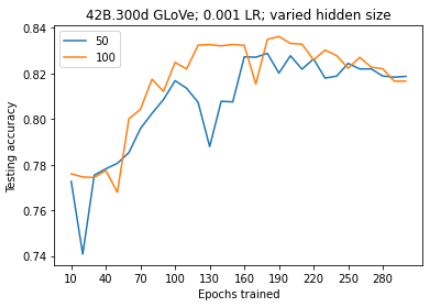
\includegraphics[width=0.75\textwidth]{images/exp-round2.png}
%% Please add the following required packages to your document preamble:
% \usepackage{booktabs}
% \usepackage{multirow}
\begin{table}[]
\begin{tabular}{@{}|c|c|c|c|c|@{}}
\toprule
\textbf{GLoVe}            & \textbf{Hidden Size} & \textbf{LR}            & \textbf{Peak Test Accuracy} & \textbf{Final Acc.} \\ \midrule
\multirow{2}{*}{42B.300d} & 50                   & \multirow{2}{*}{0.001} & 0.8289 (170 epochs)         & 0.8188              \\ \cmidrule(lr){2-2} \cmidrule(l){4-5} 
                          & 100                  &                        & 0.8363 (180 epochs)         & 0.8167              \\ \bottomrule
\end{tabular}
\label{tab:round2}
\end{table}
\end{frame}

\begin{frame}[c]
\begin{minipage}[c][\textheight][c]{\linewidth}
\centering
Thanks for your attention!
\end{minipage}
\end{frame}
\end{document}